\documentclass{article}
\usepackage{amsmath} % For math equations
\usepackage{amsfonts} % For math fonts
\usepackage{amssymb} % For math symbols
\usepackage{float}
\usepackage{enumitem}
\usepackage{graphicx}
\setlist[enumerate,1]{label=\arabic*.}
\setlist[enumerate,2]{label=\alph*.,itemindent=2em}

\title{HW 4 - 135}
\author{Asher Christian 006-150-286}
\date{1.11.24}

\begin{document}
    \maketitle
    \section{69-1}
    \[
    y' = y^2, \; \; \; y(0) = 1
    .\] 
    $y_0(x)=1$ 
    \[
    y_1(x) = y_0 + \int_{x_0}^{x}y_0(t)^2dt = 1 + \int_{0}^{x}1dt = 1 + x
    .\] 
    \begin{align*}
        y_2(x) &= 1 + \int_{0}^{x}(1+t)^2dt\\
               &= 1 +  (\frac{1}{3}(1-t)^3 \Big|_0^x)\\
               &= \frac{1}{3}(1+x)^2+\frac{2}{3}\\
               &= 1 + x + x^2 +\frac{1}{3}x^3\\
        y_3(x) &= 1 + \int_{0}^{x}(1+t+t^2+\frac{1}{3}t^{3})^2dt\\
               &= 1 + \int_{0}^{x}(1+2t+3t^2+\frac{8}{3}t^{3}+\frac{5}{3}t^{4}+\frac{2}{3}t^{5}+\frac{1}{9}t^{6})dt\\
               &= 1 + x + x^2 + x^{3} + \frac{2}{3}x^4 + \frac{1}{3}x^5 + \frac{1}{9}x^6 + \frac{1}{63}x^7
    \end{align*}
    Solving for $y$ directly using separation of variables
    $\frac{dy}{dx} = y^2 \rightarrow \int_{}^{}\frac{dy}{y^2} = \int_{}^{}dx$\\
    $-\frac{1}{y} = x + c \rightarrow y = -\frac{1}{x+c}$ with $c = -1$
    \begin{figure}[H]
        \centering
        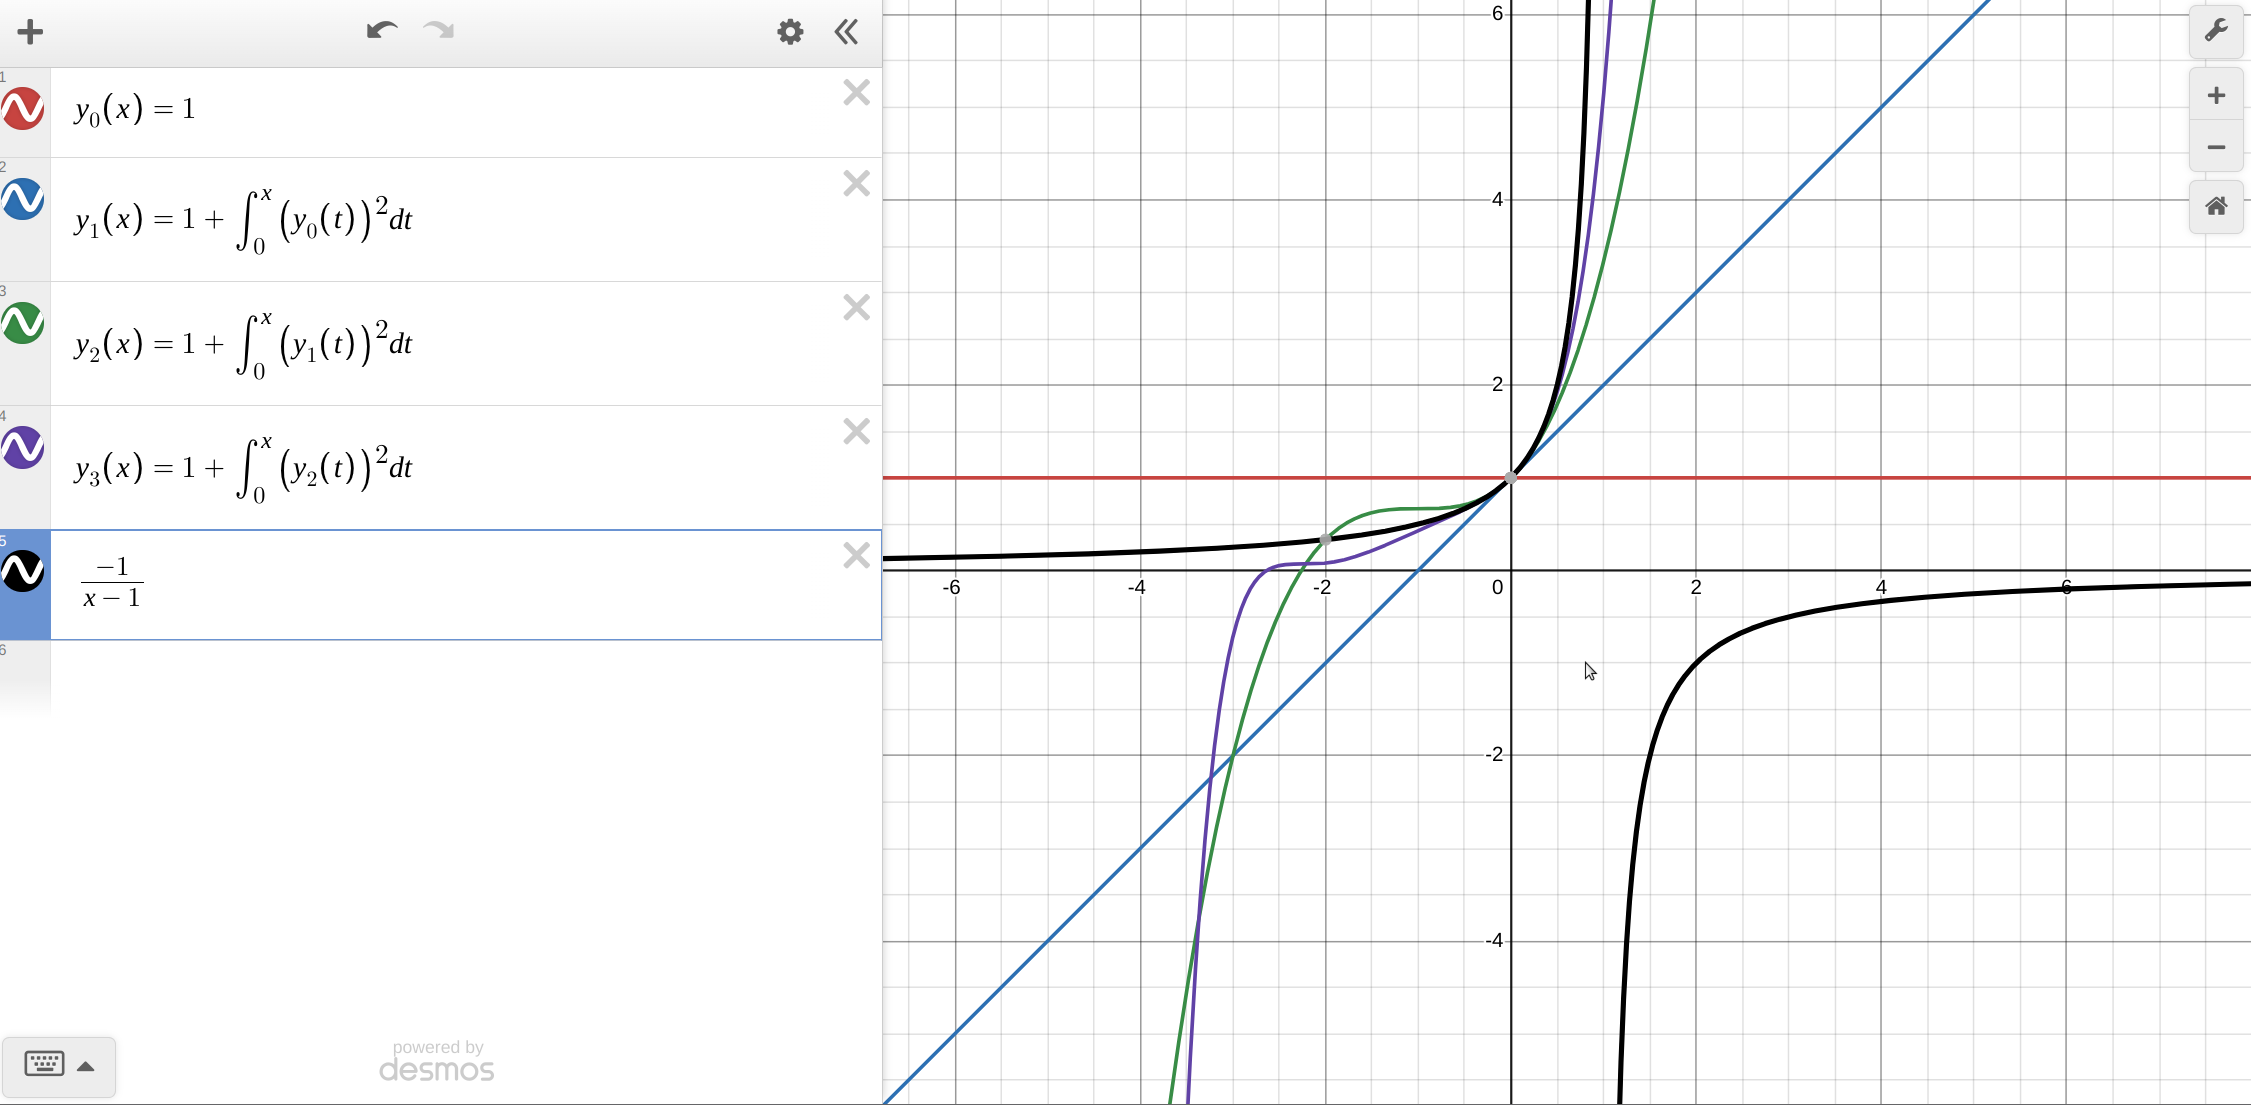
\includegraphics[width=\linewidth]{~/Documents/Math_135/HW4_1.png}
        \caption{Desmos graph of the piccard iteration and the solution to the ODE}
        \label{fig:your_label}
    \end{figure}
    \section{69-2}
    \[
    y'=2x(1+y), \; \; \; y(0) = 0
    .\] 
    $y_0(x) = 0$
    \begin{align*}
        y_1(x) &= 0 + \int_{0}^{x}(2t)dt \\
               &= x^2\\
        y_2(x) &= 0 + \int_{0}^{x}(2t(1+t^2))dt\\
               &= \int_{0}^{x}(2t+2t^3)dt\\
               &= x^2+\frac{1}{2}x^4\\
        y_3(x) &= \int_{0}^{x}(2t(1+t^2+\frac{1}{2}t^{4}))dt\\
               &= x^2+\frac{1}{2}x^{4}+ \frac{1}{6}x^{6}\\
        y_4(x) &= \int_{0}^{x}(2t(1+t^2+\frac{1}{2}t^4+\frac{1}{6}t^6))dt\\
               &= x^2+\frac{1}{2}x^{4}+\frac{1}{6}x^{6}+\frac{1}{24}x^8
    \end{align*}
    solving directly
    \begin{align*}
        y'(x) &= 2x(1+y)\\
        \int_{}^{}\frac{1}{y+1} &= \int_{}^{}2x\\
        ln(y+1) &= x^2+c\\
        y & = De^{x^2}-1
    \end{align*}
    D = 1 to satisfy initial condition.
    \begin{figure}[H]
    \centering
        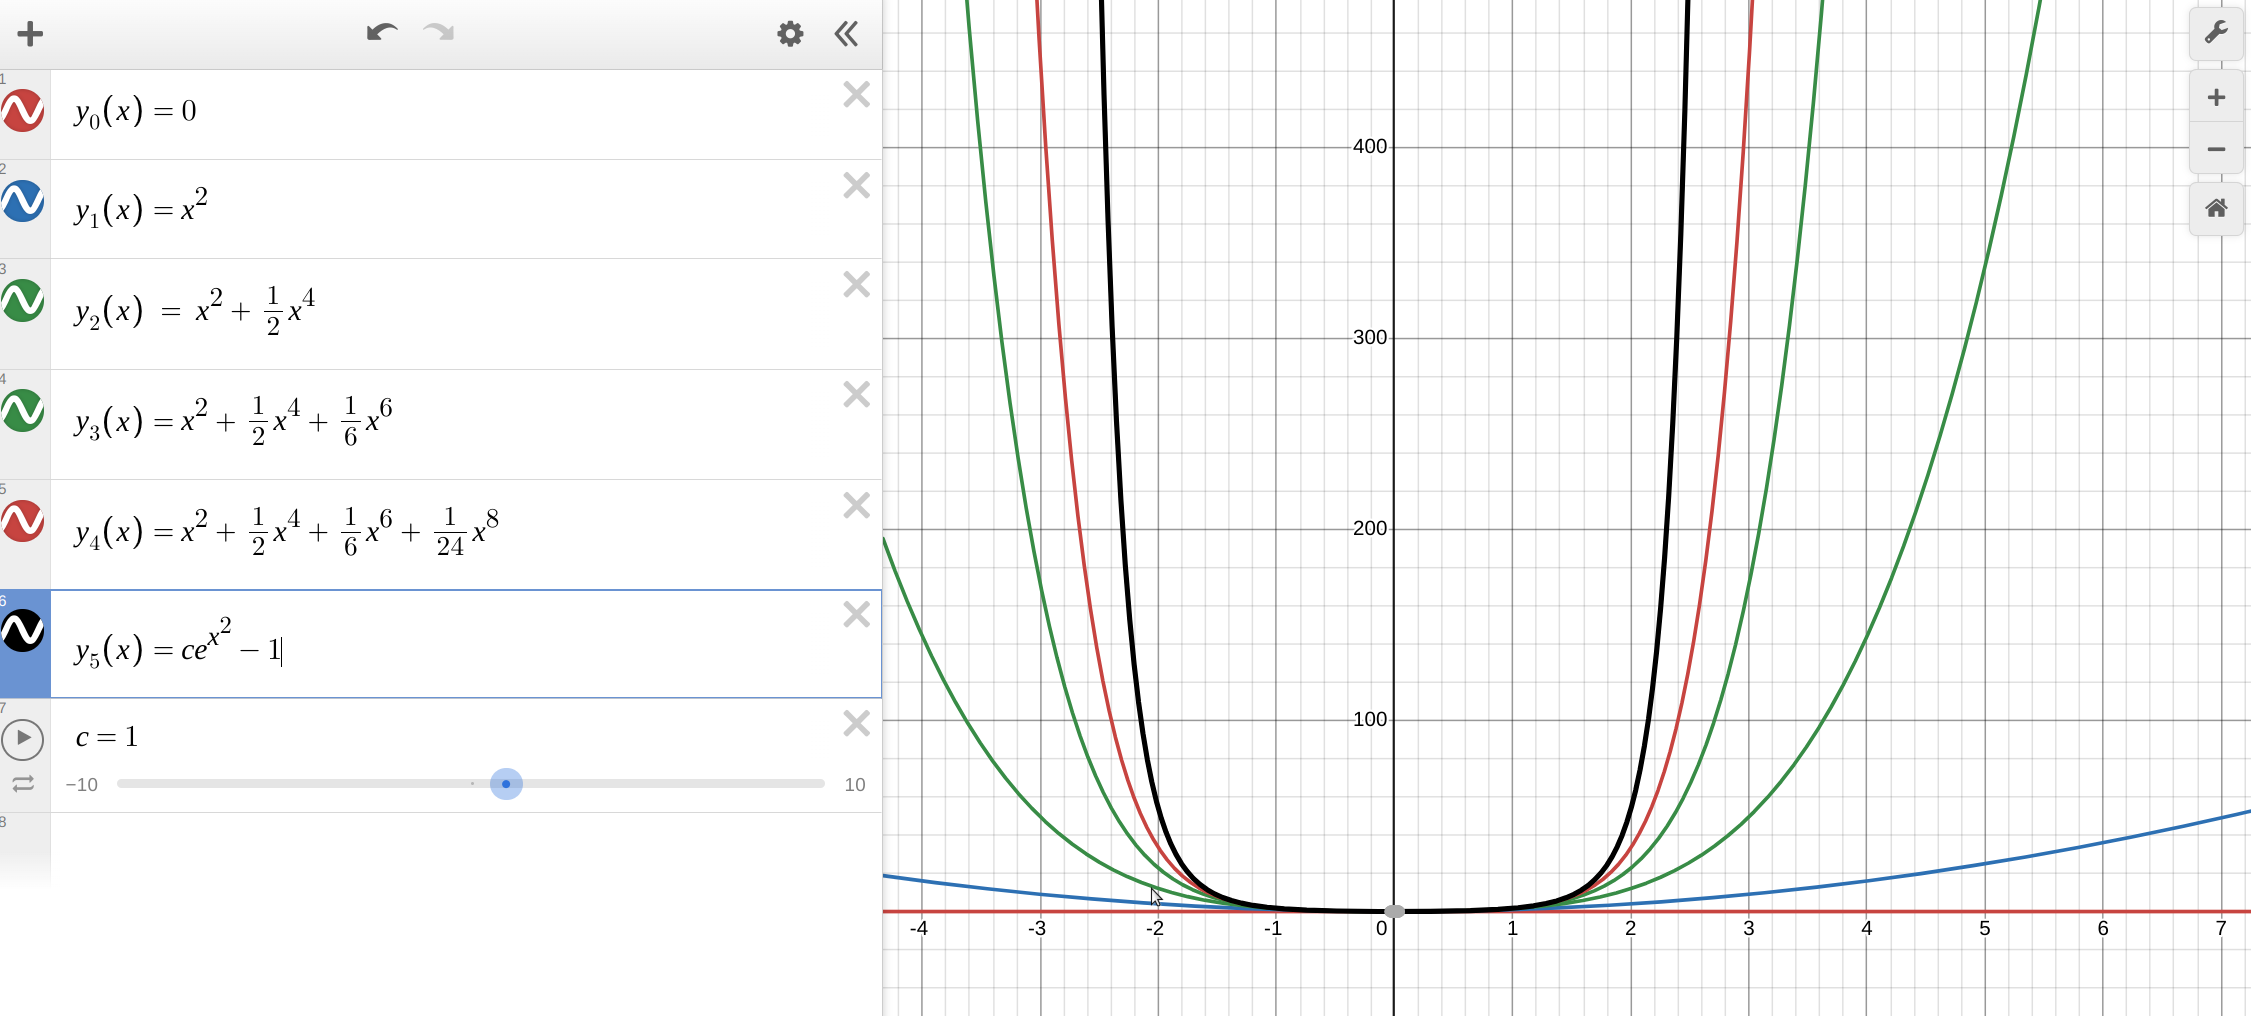
\includegraphics[width=\linewidth]{~/Documents/Math_135/HW_4_2.png}
        \caption{Comparing the first 4 iteratinos with the solution to the ODE}
        \label{fig:your_label}
    \end{figure}

    \section{69-3}
    \[
    y' = x + y, \; \; \; y(0) = 1
    .\] 
    \begin{enumerate}
        \item (a)
        \begin{align*}
            y_0 &= e^{x}\\
            y_1 &= 1 + \int_{0}^{x}(t+e^{t})dt\\
                &=  \frac{1}{2}x^2 + e^{x}\\
                &= \sum_{i=2}^{\infty}\frac{x^{i}}{i!} - x - 1 + e^{x}.\\
                &= 2e^{x}-x-1
        \end{align*}
    \item (b)
        \begin{align*}
            y_0 &= 1 + x\\
            y_1 &= 1 + \int_{0}^{x}(2t+1)dt\\
                &= 1 + x^2 + x\\
                &= \sum_{i=2}^{\infty}\frac{2x^{i}}{i!} + 1 + x\\
                &= 2\sum_{i=0}^{\infty}\frac{x^{i}}{i!} - x - 1\\
                &= 2e^{x}-x-1
        \end{align*}
    \item (c)
        \begin{align*}
            y_0 &= cos(x)\\
            y_1 &= 1 + \int_{0}^{x}(t+cos(t))dt\\
                &= 1 + \frac{1}{2}x^2 + sin(x)\\
            y_2 &= 2 + x + \frac{x^2}{2} + \frac{x^{3}}{6}-cos(x)\\
            y_3 &= 1 + 2x + x^2+  \frac{x^{3}}{6} + \frac{x^{4}}{24} - sin(x) \\
            y_4 &= x + \frac{3x^2}{2} + \frac{x^{3}}{3} + \frac{x^{4}}{24}  + \frac{x^{5}}{120} + cos(x)\\
            y^{5} &= 1 + x^2 + \frac{x^{3}}{2} + \frac{x^{4}}{12} + \frac{x^{5}}{120} + \frac{x^{6}}{720} + sin(x)\\
        \end{align*}
        This one was harder to find a pattern for because the cylce $cos \rightarrow sin \rightarrow -cos \rightarrow -sin$ produces different constant terms and different $x$ terms
        which propogate and affect the later terms but the graphs clearly approach $2e^{x}-x-1$.

    \end{enumerate}
    
    \section{70-1}
    \begin{enumerate}
        \item Theorem A guarantees a solution because $y^2$ and $2y$ are both continuous on the 
        entirety of $ \mathbb{R}^2$ but this is only for some $h$ not the entire line.
        The solution through $y(0) = 0$ is $y=0$ and the solution through $y(0) = 1$ is $y = -\frac{1}{x-1}$ which is not continuous on 
        $x = 1$. and the function
        \[
        f(x) = 
        \begin{cases}
            -\frac{1}{x-1} & \text{ if} x \le 1 \\
            0 & \text{if } x > 1
        \end{cases}
        .\] 
        Satisfies the same requirements
    \end{enumerate}
    \section{70-2}
    \begin{enumerate}
        \item (a) 
            $\frac{\partial f}{\partial y} = \frac{1}{2}y^{-\frac{1}{2}}$
            The partial gets arbitrarily large at values close to zero so bounding the partial is impossible.
            For example any $K$ that bounds it take $y_1 = \frac{1}{4}$ and $y_0 = (\frac{1}{2K+1})^2$ and the difference is strictly greater than $K$.
        \item (b)
            For any bound on y greater than $0$ we know that the partial of $y$ is strictly decreasing because the second derivative is negative for all positive $y$.
            The maximum distance is then taken as the partial evaluated at c and the partial evaluated at the right bound d and their difference is necessarily the largest
            difference between partial values.
    \end{enumerate}




    
\end{document}
